% !TEX root = ./Basilisk-thrFiringSchmitt-2019-03-29.tex


\begin{figure}[h]
	\centerline{
		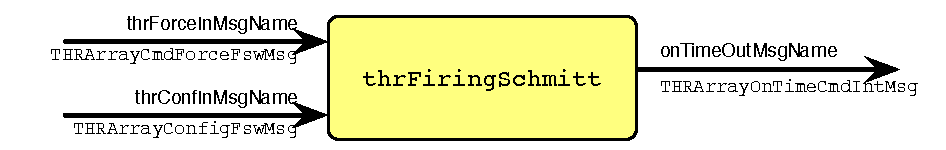
\includegraphics{Figures/moduleImg}
	}
	\caption{Illustration of the module input and output messages.}
	\label{fig:moduleImg}
\end{figure}


\section{Model Description}
This module implements a Schmitt trigger thruster firing logic.  More details can be found in Reference~\citenum{Alcorn:2016rz}.    Here if the minimum desired on-time $t_{\text{min}}$ is specified.  If the commanded on-time $t_{i}>t_{\text{min}}$ then the thruster is turned off for the duration of $t_{i}$.  If $t_{i}< t_{\text{min}}$ then the Schmitt trigger logic is invoked.  Let $l$ be the current thruster duty cycle relative to this minimum thruster firing time.
$$
	l = \frac{t_{i}}{t_{\text{min}}}
$$
If $l$ is larger than a threshold $l_{\text{on}}$ then the thruster control time is set to $t_{i} = t_{\text{min}}$.  Once on, the thruster level must drop below a lower threshold $l_{\text{off}}$ to turn off again.  The benefit of this logic is that it provides a good balance between fuel efficiency and pointing accuracy.  


\subsection{Module Input and Output Messages}
As illustrated in Figure~\ref{fig:moduleImg}, the module reads in two messages.  One message contains the thruster configuration message from which the maximum thrust force value for each thruster is extracted and stored in the module.  This message is only read in on {\tt Reset()}.  

The second message reads in an array of requested thruster force values with every {\tt Update()} function call.  These force values $F_{i}$ can be positive if on-pulsing is requested, or negative if off-pulsing is required.  On-pulsing is used to achieve an attitude control torque onto the spacecraft by turning on a thruster.  Off-pulsing assumes a thruster is nominally on, such as with doing an extended orbit correction maneuver, and the attitude control is achieved by doing periodic off-pulsing.  

The output of the module is a message containing an array of thruster on-time requests.  If these on-times are larger than the control period, then the thruster remains on only for the control period upon which the on-criteria is reevaluated.  


\subsection{Reset() Functionality}
\begin{itemize}
	\item The control period is dynamically evaluated in the module by comparing the current time with the prior call time.  In {\tt reset()} the {\tt prevCallTime} variable is reset to 0.  
	\item The thruster configuration message is read in and the number of thrusters is stored in the module variable {\tt numThrusters}.  The maximum force per thruster is stored in {\tt maxThrust}.
	\item The last thruster state variable {\tt lastThrustState} is set to off (i.e. false)
\end{itemize}

\subsection{Update() Functionality}
The goal of the {\tt update()} method is to read in the current attitude control thruster force message and map these into a thruster on-time output message using the Schmitt trigger logic.\cite{Alcorn:2016rz}  The module sets a desired minimum thruster on time $t_{\text{min}}$.  This is typically not set to the lower limit of the thruster resolution, but rather to a value that provides a good duty cycle and avoids excessive short on-off switching.   The cost naturally is a reduced pointing capability.  Let the duty cycle $l$ be defined as the ratio between the commanded on time $t_{i}$ and $t_{\text{min}}$.  The thruster is turned on for a period $t_{i} = t_{\text{min}}$ if $l$ is larger than  $l_{\text{on}}$.  The thruster then remains on until $l$ drops below a lower threshold $l_{\text{off}}$.  The benefit of this method is that it provides a good balance between fuel usage and pointing accuracy.\cite{Alcorn:2016rz}


If the {\tt update()} method is called for the first time after reset, then there is no knowledge of the control period $\Delta t$.  In this case the thruster on-time values are set either to 0 (on-pulsing case) or 2 seconds (off-pulsing case).  After writing out this message the module is exited.  This logic is essence turns off the thruster-based attitude control for one control period. 

If this is a repeated call of the {\tt update()} method then the control period $\Delta t$ is evaluated by differencing the current time with the prior call time.  Next a loop goes over each installed thruster to map the requested force $F_{i}$ into an on-time $t_{i}$.  The following logic is used.  
\begin{itemize}
	\item If off-pulsing is used then $F_{i}\le 0$ and we set $$F_{i} += F_{\text{max}}$$ to a reduced thrust to achieve the negative $F_{i}$ force.  
	\item Next, if $F_{i} < 0$ then it set to be equal to zero.  This can occur if an off-pulsing request is larger than the maximum thruster force magnitude $F_{\text{max}}$.  
	\item The nominal thruster on-time is computed using $$t_{i}  = \dfrac{F_{i}}{F_{\text{max}}} \Delta t$$ 
	\item If $\Delta t > t_{i} \ge t_{\text{min}}$ the thruster on time is set to $t_{i}$
	\item If $t_{i} > \Delta t$ then the thruster is saturated.   In this case the on-time is set to $t_{i} = 1.1\Delta t$ such that the thruster remains on through the control period.
	\item The Schmitt trigger logic occurs if $t_{i} < t_{\text{min}}$.  If $l>l_{\text{on}}$ then $t_{i} = t_{\text{min}}$.  This command of $t_{i} = t_{\text{min}}$ remains on as long as $l > l_{\text{off}}$.  If $l<l_{\text{off}}$ then $t_{i} = 0$ and the thruster is turned off again for the control period.
	\item The final step is to store the thruster on-time into  and write out this output message
\end{itemize}


